\chapter{Introduction}
\label{cha:Intro}

\section{Field of Research}

Fractal geometry is an area of mathematical research that concerns itself with mathematically describing n-dimensional geometries - limited here to geometries on a plane - that display \textit{interesting} characteristics. 

Figure \ref{fig:flosnek} shows a rendering of one such geometry called \textsc{Gosper's flowsnake}.
It is a single, uninterrupted curve on a triangular grid, which is

\begin{description}
	\item [self similar] The macroscopic behaviour of the curve is the same as its microscopic behaviour
	\item [self avoiding] The curve is made from one continuous line that never intersects with itself.
	\item [edge covering] The curve travels across every cell of its grid, i.e. it fills up a given, arbitrary area completely
	\item [plane filling] The curve grows outward on the 2D plane without bounds. Infinitely iterated it covers the full plane.
\end{description}

\begin{figure}[h]
\centering
\begin{subfigure}{.33\textwidth}
  \centering
  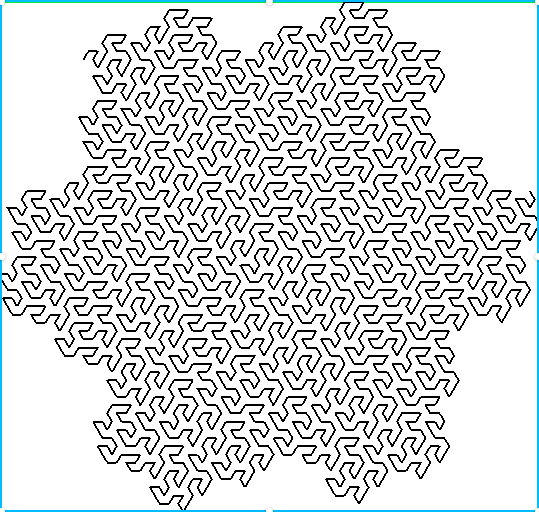
\includegraphics[width=.7\linewidth]{flosnek_4it}
  \caption{4 iterates}
\end{subfigure}%
\begin{subfigure}{.33\textwidth}
  \centering
  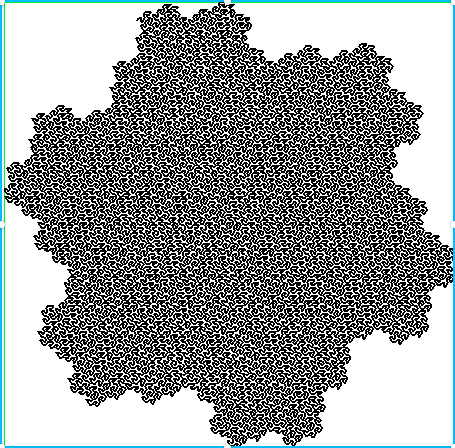
\includegraphics[width=.7\linewidth]{flosnek_5it}
  \caption{5 iterates, rescaled}
\end{subfigure}%
\begin{subfigure}{.33\textwidth}
  \centering
  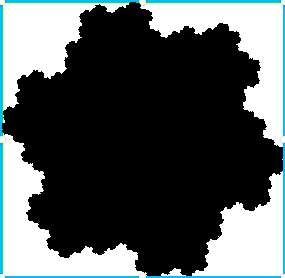
\includegraphics[width=.7\linewidth]{flosnek_8it}
  \caption{8 iterates, rescaled}
\end{subfigure}
\caption{Rendering of \textsc{Gosper's flowsnake}, with \gls{bounding box}}
	\label{fig:flosnek}
\end{figure}

The curve is obtained by iterating a so-called \gls{lsys}.

Originally introduced by biologist \textsc{Aristid Lindenmayer} in 1968 "as a foundation for an axiomatic theory of development" of plants \citep[Preface]{Prusinkiewicz2013}, it was found to be a useful language for describing a wide class of fractal geometries.
An \gls{lsys} consists of an inital string - the \textit{\gls{axiom}} - which is manipulated via a set of substitution \textit{rules}, the result of which is a called the first \textit{production} or \textit{iterate} of the \gls{lsys}. Subsequent iterations are generated by applying the \textit{rules} to the current \textit{production}.

The \gls{lsys} for figure \ref{fig:flosnek} is given in \citet[p.7]{Arndt2016} to be 
\begin{quote}
	\centering
	L $\rightarrow$ L+R++R-L- -LL-R+ \quad and \quad R $\rightarrow$ -L+RR++R+L- -L-R
\end{quote}
starting with an \textit{\gls{axiom}} of L. The first iterate of \textsc{Gosper's flowsnake} thus becomes L+R++R-L- -LL-R+, as the initial \gls{axiom} L gets substituted as per the left rule. 

The characters in this string are given special meaning w.r.t. to the curve:
\begin{description}
	\item[Alphabetic character] Denotes drawing a line from the current position forward by on a defined length. Forward being defined as the current direction
	\item[+ -] Characters denoting changes in direction by a set amount, e.g. in figure \ref{fig:flosnek} by $\pm60^\circ$, creating a triangular grid of movement
\end{description}

Those rules define a way to render a curve given by a \textit{\gls{product}}, and can be extended by other, auxilliary characters, discussed in \ref{sec:implementation}, e.g. \_ which changes color of subsequent segments.

\begin{figure}[hb]
	\centering
	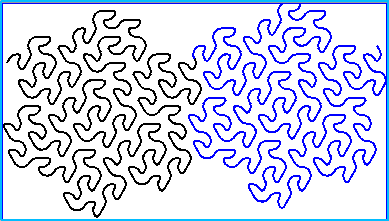
\includegraphics[width=0.5\textwidth]{flosnek_color}
	\caption{3-iterate rendering of \textsc{Gosper's flowsnake} with axiom \textrm{L\_L} and a rounding factor of 0.5}
\end{figure}

\section{Problem Statement}
In 2016, Prof. Jörg Arndt, the supervisor of this thesis, conducted research on finding plane-filling curves for \gls{lsys} with one non-constant character and published an article \citep{Arndt2016}, where he presented 2D renderings of the curves found.

The tools used to get from an \gls{lsys} description to a graphical, pdf-embeddable rendering of the iterated curve were assortments of chained commandline scripts, leaving much to be desired in flexibility and ease-of-use.

Thus, a request was issued for the creation of a \emph{cross-platform, maintainable and extensible} software that is able to create, visualize and export \gls{pfc}s from their \gls{lsys} descriptions.

\section{Approach}

Since this problem is multi-faceted, and the additional requirements introduce significant complexity on top of the "implement a renderer/exporter" core task, a structured approach to finding a solution is taken using decomposition methods from software engineering.

First, the requirements are formulated and discussed.

Then, research is conducted on available technologies for satisfying given requirements.

An architectural model is created using \gls{uml} to define the system architecture.

This model ist then implemented and refined/amended to address issues arising during the implementation process.

The software is tested during development with \gls{ci} and \gls{unit test} techniques.

Finally, a short investigation of application performance is conducted.

\section{Requirements to a Solution}
The following requirements to a satisfactory solution are given in figure \ref{fig:directreq} with a supposed workflow shown in the use-case diagram \ref{fig:uc}

\begin{figure}[h]
	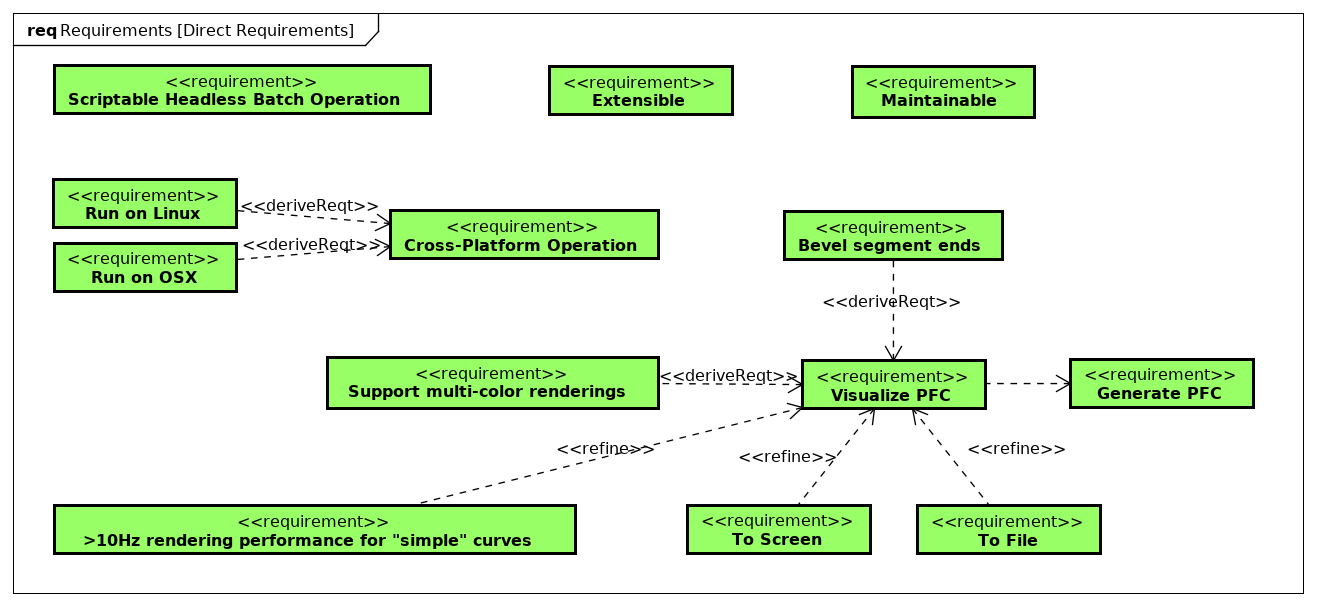
\includegraphics[width=\textwidth]{DirectRequirements}
	\caption{Direct user requirements to a solution}
	\label{fig:directreq}
\end{figure}


\begin{figure}
	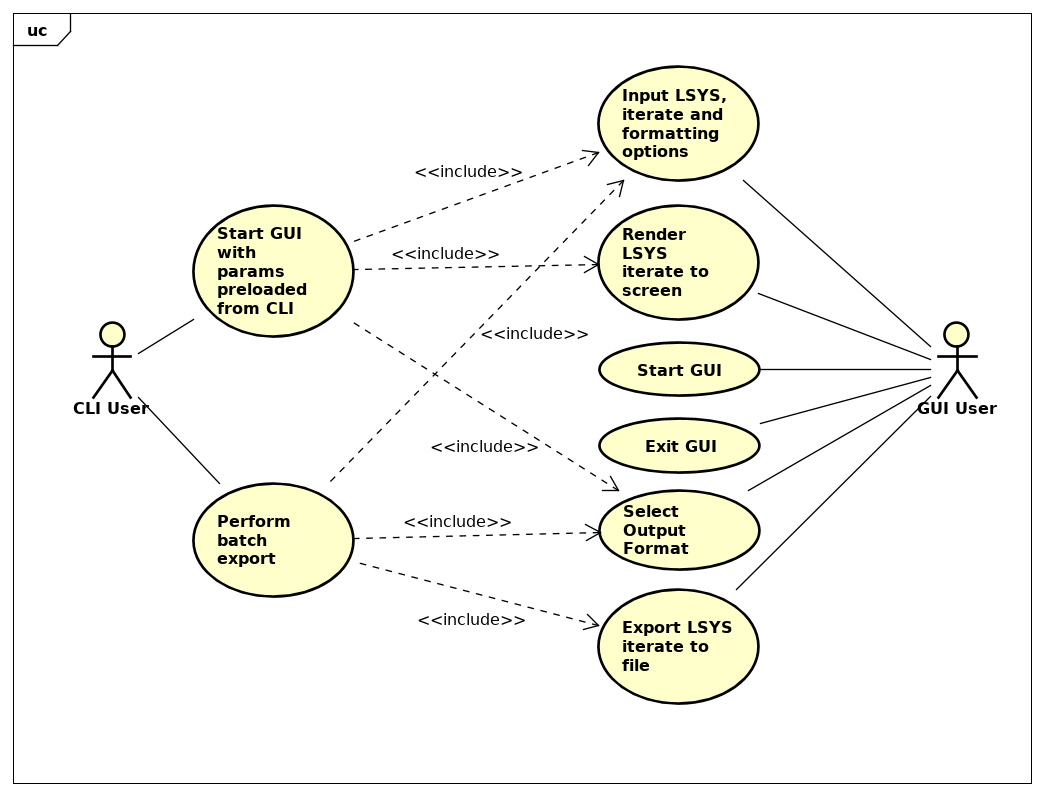
\includegraphics[width=\textwidth]{UseCaseDiagram}
	\caption{Workflow with the pfcrender tool}
	\label{fig:uc}
\end{figure}

These requirements are discussed in detail in the following sections and an architecture is formulated that satisfies them.
